\documentclass[11pt]{article}
\usepackage[utf8]{inputenc}
\usepackage[T1]{fontenc}
\usepackage{geometry}
\usepackage{amsmath,amssymb,amsthm}
\usepackage{algorithm}
\usepackage{algorithmic}
\usepackage{graphicx}
\usepackage{subcaption}
\usepackage{booktabs}
\usepackage{array}
\usepackage{multirow}
\usepackage{longtable}
\usepackage{rotating}
\usepackage{pdflscape}
\usepackage{afterpage}
\usepackage{capt-of}
\usepackage{float}
\usepackage{hyperref}
\usepackage{cleveref}
\usepackage{listings}
\usepackage{xcolor}
\usepackage{tikz}
\usepackage{pgfplots}
\pgfplotsset{compat=1.17}

\geometry{margin=1in}

% Custom colors
\definecolor{codegreen}{rgb}{0,0.6,0}
\definecolor{codegray}{rgb}{0.5,0.5,0.5}
\definecolor{codepurple}{rgb}{0.58,0,0.82}
\definecolor{backcolour}{rgb}{0.95,0.95,0.92}

% Code listing style
\lstdefinestyle{mystyle}{
    backgroundcolor=\color{backcolour},
    commentstyle=\color{codegreen},
    keywordstyle=\color{magenta},
    numberstyle=\tiny\color{codegray},
    stringstyle=\color{codepurple},
    basicstyle=\ttfamily\footnotesize,
    breakatwhitespace=false,
    breaklines=true,
    captionpos=b,
    keepspaces=true,
    numbers=left,
    numbersep=5pt,
    showspaces=false,
    showstringspaces=false,
    showtabs=false,
    tabsize=2
}
\lstset{style=mystyle}

% Title information
\title{\textbf{Sports Tournament Scheduling: \\
A Multi-Paradigm Optimization Approach}}

\author{
Leonardo Tassinari \\
Student ID:   \\
\\
Francesco Zattoni \\
Student ID:   \\
\\
\textit{Combinatorial Decision Making and Optimization} \\
\textit{University of Bologna} \\
\textit{Academic Year 2024-2025}
}

\date{July 2025}

\begin{document}

\maketitle

\tableofcontents
\newpage

\section{Introduction}

This report presents a comprehensive study of the Sports Tournament Scheduling (STS) problem, focusing on the development and comparison of multiple optimization models. The aim is to provide a unified framework for modeling, analyzing, and solving the STS problem, enabling a fair and systematic evaluation of different solution paradigms. All models considered in this work share a common formalization, which is described in this section.

\subsection{Common Model Formalization}

\paragraph{Input Parameters.}
The STS problem is defined by the following parameters, which are common to all models:
\begin{itemize}
    \item $n$: Number of teams (even integer)
    \item $w = n-1$: Number of weeks
    \item $p = n/2$: Number of periods (matches per week)
    \item Teams are indexed by $t \in \{1, 2, \ldots, n\}$
    \item Weeks are indexed by $w \in \{1, 2, \ldots, n-1\}$
    \item Periods are indexed by $p \in \{1, 2, \ldots, n/2\}$
\end{itemize}

\paragraph{Objective Variable and Bounds.}
For the optimization variant, the objective is to minimize the maximum imbalance in home and away games for any team:
\[
M = \max_{t \in \{1, \ldots, n\}} |h_t - a_t|
\]
where $h_t$ and $a_t$ denote the number of home and away games played by team $t$, respectively. The upper bound for $M$ is $n-1$, even if the practical upper bound is lower, because it's impossible that every team plays only away games or home games. The theoretical lower bound for $M$ is $1$ for even $n$, since $h_t$ and $a_t$ cannot be equal.

\paragraph{Constraints.}
All models enforce the following core constraints:
\begin{enumerate}
    \item Each pair of teams plays exactly once during the tournament.
    \item Each team plays exactly once per week.
    \item Each period in each week hosts exactly one match.
    \item No team plays against itself.
    \item Each team appears in the same period at most twice across all weeks.
\end{enumerate}

\paragraph{Pre-processing and Symmetry Breaking.}
To improve solver efficiency, all models may include pre-processing steps such as:
\begin{itemize}
    \item Translating the model into a solver-independent language (such as DIMACS or SMT-LIB), which may require additional pre-processing time before the actual solving phase. 
    \item Fixing the schedule of the first week to break team symmetries.
    \item Lexicographic ordering of weeks and/or periods to break week and period symmetries.
    \item Adding implied constraints (e.g., total matches per team).
\end{itemize}

\section{CP model}

\subsection{Decision Variables}

The MiniZinc CP model represents the tournament schedule using two primary arrays of integer decision variables:

\begin{itemize}
    \item \textbf{home[$w$, $p$]}: For each week $w \in \{1, \ldots, n-1\}$ and period $p \in \{1, \ldots, n/2\}$, \texttt{home[$w$, $p$]} is an integer variable indicating the team assigned as the home team in that slot.
    \item \textbf{away[$w$, $p$]}: For each week $w \in \{1, \ldots, n-1\}$ and period $p \in \{1, \ldots, n/2\}$, \texttt{away[$w$, $p$]} is an integer variable indicating the team assigned as the away team in that slot.
\end{itemize}

Both variables take values in $\{1, \ldots, n\}$ and together define the assignment of teams to each match in the tournament schedule. All additional variables and constraints in the model are defined in terms of these primary decision variables, as described in the common formalization. \\
Another design of the decision variables was tested: \texttt{matches}, an array for each possible match ID that takes values in $\{1..slots\},\ slots = (n-1)\times(n/2)$, but it led to a more complex implementation with not-so-evident improvements only for $n=12$. Also, the addition of channeling constraints between \texttt{matches}, \texttt{home} and \texttt{away} didn't help.

\subsection{Objective Function}

The objective variable and its theoretical bounds are described in Section~1. In the MiniZinc model, the objective is implemented as the variable \texttt{max\_diff}, which represents the maximum absolute difference between the number of home and away games for any team:
\[
\texttt{max\_diff} = \max_{t \in \text{Teams}} \left|\,\texttt{home\_count}[t] - \texttt{away\_count}[t]\,\right|
\]
where the auxiliary variables \texttt{home\_count}[t] and \texttt{away\_count}[t] are defined as follows:
\begin{itemize}
    \item \texttt{home\_count}[t]: the total number of times team $t$ appears as the home team across all weeks and periods,
    \[
    \texttt{home\_count}[t] = \sum_{w \in \text{Weeks}} \sum_{p \in \text{Periods}} [\texttt{home}[w,p] = t]
    \]
    \item \texttt{away\_count}[t]: the total number of times team $t$ appears as the away team across all weeks and periods,
    \[
    \texttt{away\_count}[t] = \sum_{w \in \text{Weeks}} \sum_{p \in \text{Periods}} [\texttt{away}[w,p] = t]
    \]
\end{itemize}

The auxiliary variables \texttt{home\_count}[t] and \texttt{away\_count}[t] are computed efficiently using the \texttt{global\_cardinality} constraint in MiniZinc.

The model minimizes \texttt{max\_diff} using the following directive:
\begin{verbatim}
solve minimize max_diff;
\end{verbatim}

\subsection{Constraints}

\paragraph{Main Problem Constraints}

\begin{itemize} 
    \item \textbf{Each pair of teams plays exactly once.}  
    For every unordered pair of distinct teams $(i, j)$, there must be exactly one match where $i$ plays against $j$ (either as home or away):
    \begin{equation*}
        \sum_{w \in \text{Weeks}} \sum_{p \in \text{Periods}} \left( [\texttt{home}[w,p] = i \land \texttt{away}[w,p] = j] + [\texttt{home}[w,p] = j \land \texttt{away}[w,p] = i] \right) = 1
    \end{equation*}

    \item \textbf{Each team plays exactly once per week.}  
    In every week $w$, each team must appear exactly once, either as home or away. This is enforced by requiring that all teams assigned in week $w$ are distinct:
    \begin{equation*}
        \text{The set } \{\texttt{home}[w,p],\ \texttt{away}[w,p] : p \in \text{Periods}\} \text{ contains all teams without repetition.}
    \end{equation*}
    This constraint is implemented using \texttt{all\_different} for every week $w$.

    \item \textbf{Each team appears in the same period at most twice.}  
    To model this constraint, we define the variable \texttt{period\_count}[t, p] as follows:
    \begin{equation*}
        \texttt{period\_count}[t, p] = \sum_{w \in \text{Weeks}} \left( [\texttt{home}[w,p] = t] + [\texttt{away}[w,p] = t] \right)
    \end{equation*}
    This expression is implemented in MiniZinc using the \texttt{global\_cardinality} constraint, used to enforce the final constraint as:
    \begin{equation*}
        \texttt{period\_count}[t, p] \leq 2
    \end{equation*}
\end{itemize}


\paragraph{Implied Constraints}
These constraints are semantically redundant, but they can be useful to reduce the search space.

\begin{itemize}
    \item \textbf{Total matches per team:}  
    Each team $t$ must play exactly $n-1$ matches in total (as home or away):
    \begin{equation*}
        \texttt{home\_count}[t] + \texttt{away\_count}[t] = n - 1
    \end{equation*}

    \item \textbf{Total period appearances per team:}  
    Each team $t$ must appear in some period exactly $n - 1$ times over the tournament, exploiting the previously defined variable \texttt{period\_count}:
    \begin{equation*}
        \sum_{p \in \text{Periods}} \texttt{period\_count}[t, p] = n - 1
    \end{equation*}
\end{itemize}

\paragraph{Symmetry Breaking Constraints}

The STS problem exhibits several symmetries (e.g., relabeling teams, reordering weeks or periods) that can lead to redundant search. Symmetry breaking constraints reduce the number of equivalent solutions and improve solver efficiency:

\begin{itemize}
    \item \textbf{Week symmetry:}  
    Weeks can be permuted without changing the problem. To break this symmetry, we impose lexicographic ordering between consecutive weeks:
    \begin{equation*}
        (\texttt{home}[w,1], \ldots, \texttt{home}[w,p], \texttt{away}[w,1], \ldots, \texttt{away}[w,p]) <_{\text{lex}} (\texttt{home}[w+1,1], \ldots, \texttt{away}[w+1,p])
    \end{equation*}
    for all $w \in \{1, 2, \ldots, n-2\}$.

    \item \textbf{Period symmetry:}  
    Periods within a week can be permuted. We enforce lexicographic ordering between periods:
    \begin{equation*}
        (\texttt{home}[1,p], \ldots, \texttt{home}[w,p], \texttt{away}[1,p], \ldots, \texttt{away}[w,p]) <_{\text{lex}} (\texttt{home}[1,p+1], \ldots, \texttt{away}[w,p+1])
    \end{equation*}
    for all $p \in \{1, 2, \ldots, n/2-1\}$.

    \item \textbf{Team symmetry:}  
    Teams can be relabeled. We fix the first week schedule to a canonical order:
    \begin{equation*}
        \texttt{home}[1, i] = 2i - 1,\quad \texttt{away}[1, i] = 2i
    \end{equation*}
    for all $p$ in periods.
    \\
    This approach was already used for a similar problem, as shown in \cite{teamsymm}.
\end{itemize}

\subsection{Validation}

To validate the MiniZinc model, we conducted a systematic experimental study using two different solvers: \textbf{Gecode} and \textbf{Chuffed}. Both solvers were run on the same set of problem instances to allow for a fair comparison. The experiments were designed to assess the impact of symmetry breaking and implied constraints, as well as the effect of different search strategies.

\paragraph{Experimental Design}
The validation of the MiniZinc model was performed using the two already mentioned solvers with common search strategies: \texttt{first\_fail} heuristic to select the variable with the smallest domain, \texttt{relax\_and\_reconstruct(85)} to escape local minima by fixing $85\%$ of the found solution and reconstructing the remaining part of it. \\One search strategy differs per solver: Gecode employed also the \texttt{indomain\_random} to assign a randomly chosen value from the selected variable; Chuffed was tested using \texttt{indomain\_min}, as \texttt{indomain\_random} is not supported. \\
Restart strategies were tried with Gecode because of the available randomization, but they didn't help the search, so they were not included in the final table results.\\
TODO Experiments were conducted on a machine with an Intel Core i7 processor and 16GB RAM, running MiniZinc 2.9.3 with Gecode 6.3.0 and Chuffed 0.13.2 on a Docker container from Ubuntu 22.04.\\
For each instance, we evaluated the following configurations:
\begin{itemize}
    \item Chuffed and Gecode with/without symmetry breaking constraints,
    \item Chuffed and Gecode with/without implied constraints,
    \item Chuffed and Gecode with/without search strategies.
\end{itemize} 
Also, other strategies were used, but they didn't improve either the performance or the complexity of the implemented model: we tried \texttt{bounds} and \texttt{domain} to make the solver use specific kinds of constraint propagation; a change in the order of the variables, i.e. swapping the weeks with the periods in both \texttt{home} and \texttt{away} arrays.

\paragraph{Experimental Results}

The results obtained using the described search strategies are reported in the following tables and in the Chuffed plot to assess the effectiveness of symmetry breaking constraints, implied constraints, and search strategies.

\begin{table}[H]
\label{tab:chuffed}
\small
\begin{tabular}{@{}lcccccc@{}}
\toprule
ID & Chuffed + SB & Chuffed w/o SB & Chuffed + IC & Chuffed w/o IC & Chuffed + SS & Chuffed w/o SS \\
\midrule
6 & 100 & 120 & 80 & 80 & 80 & 80\\
8 & 50 & 60 & \texttt{N/A} & \texttt{N/A} & 80 & 80 \\
10 & \texttt{UNSAT} & \texttt{UNSAT} & \texttt{N/A} & \texttt{N/A} & 80 & 80\\
12 & \texttt{UNSAT} & \texttt{UNSAT} & \texttt{N/A} & \texttt{N/A} & 80 & 80\\
14 & \texttt{UNSAT} & \texttt{UNSAT} & \texttt{N/A} & \texttt{N/A} & 80 & 80\\
\bottomrule
\end{tabular}
\caption{Results using Chuffed with the possible combinations of active constraints.}
\end{table}

\begin{table}[H]
\centering
\small
\label{tab:search}
\begin{tabular}{@{}lcccccc@{}}
\toprule
ID & Gecode + SB & Gecode w/o SB & Gecode + IC & Gecode w/o IC & Gecode + SS & Gecode w/o SS \\
\midrule
6 & 100 & 120 & 80 & 80 & 80 & 80\\
8 & 50 & 60 & \texttt{N/A} & \texttt{N/A} & 80 & 80 \\
10 & \texttt{UNSAT} & \texttt{UNSAT} & \texttt{N/A} & \texttt{N/A} & 80 & 80\\
12 & \texttt{UNSAT} & \texttt{UNSAT} & \texttt{N/A} & \texttt{N/A} & 80 & 80\\
14 & \texttt{UNSAT} & \texttt{UNSAT} & \texttt{N/A} & \texttt{N/A} & 80 & 80\\
\bottomrule
\end{tabular}
\caption{Results using Gecode with the possible combinations of active constraints.}
\end{table}

\begin{figure}[H]
    \centering
    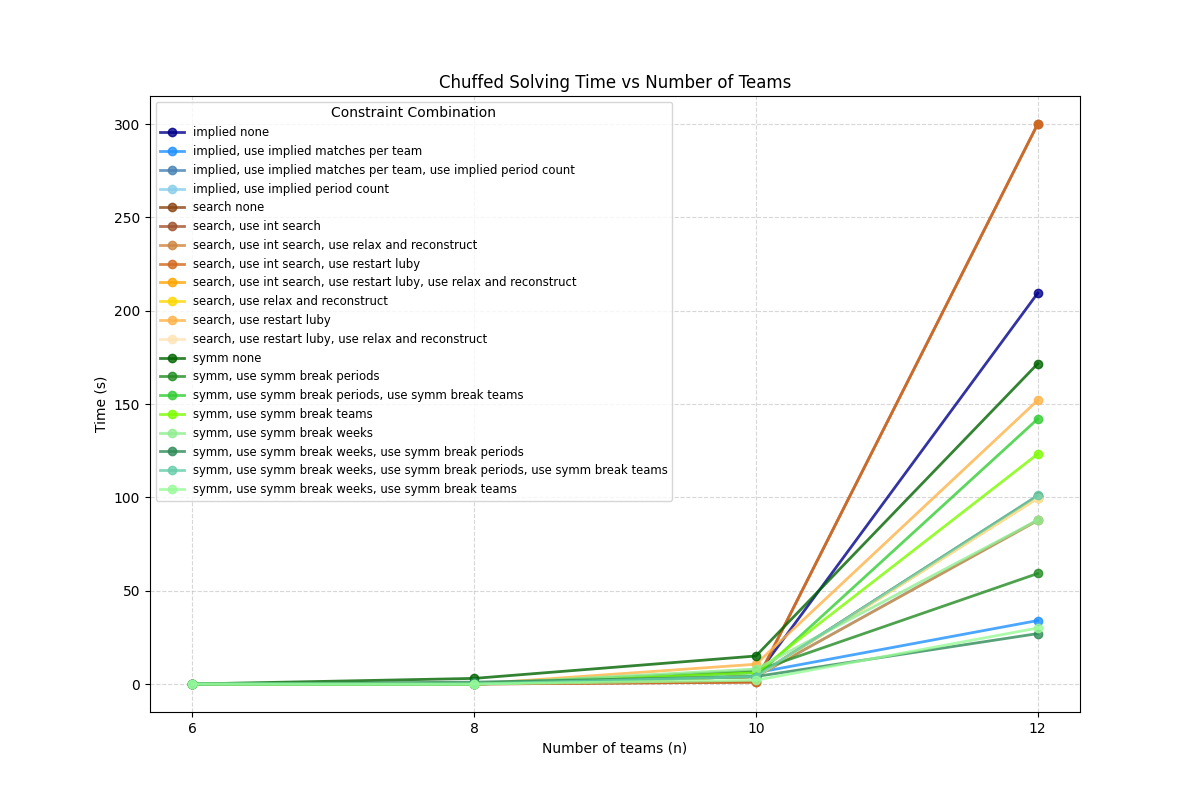
\includegraphics[width=1\textwidth]{chuffed_plot.png}
    \caption{Chuffed solver: solving time for different constraint configurations.}
    \label{fig:chuffed_plot}
\end{figure}

\section{SAT Model}

\subsection{Decision variables}
The core decision variables in the SAT model are 3D arrays: 
\begin{itemize}
    \item \textbf{home[$w$, $p$, $t$]}: Boolean variables where \textbf{home[$w$, $p$, $t$]} is true if and only if team $t$ plays at home in week $w$ during period $p$.

\textbf{away[$w$, $p$, $t$]}: Boolean variables where \textbf{away[$w$, $p$, $t$]} is true if and only if team $t$ plays away in week $w$ during period $p$.
\end{itemize}
Other auxiliary variables are added for the encodings of the cardinality constraints, that will be discussed in Section~3.3.

\subsection{Objective Function}

To optimize an objective function in SAT we use a \emph{binary search} approach over possible values of the objective. For each candidate value, we encode the constraint ``no team has a home/away imbalance greater than $d$'' as SAT clauses, and check satisfiability.
\\The objective is:
\[
\min \max_{t} |H_t - A_t|
\]
Since $H_t + A_t = w$ for all $t$, minimizing $|H_t - A_t|$ is equivalent to bounding $H_t$ within $[\lfloor w/2 \rfloor - d/2, \lceil w/2 \rceil + d/2]$ for some $d$.
\\
The sum $H_t = \sum_{w,p} \textbf{home[$w$, $p$, $t$]}$ is the number of home games for team $t$.
To enforce the objective, for a given candidate $d$, we add for each team $t$:
\[
\texttt{min\_home} \leq H_t \leq \texttt{max\_home}
\]
where
\[
\texttt{min\_home} = \max\left(0, \frac{w - d}{2}\right), \quad
\texttt{max\_home} = \min\left(w, \frac{w + d}{2}\right)
\]
During the binary search, $d$ becomes smaller, approaching $1$, then \texttt{min\_home} and \texttt{max\_home} approach $w/2$, leading to a more balanced scheduling.

\subsection{Constraints}

\paragraph{Main Problem Constraints}
\begin{itemize}
    \item \textbf{Each slot has exactly one home and one away team, and they are different:}
    \begin{align*}
        &\forall w, p: \quad \texttt{exactly\_one}(\{\forall t: \space \textbf{home[$w$, $p$, $t$]}\}) \\
        &\forall w, p: \quad \texttt{exactly\_one}(\{\forall t: \space \textbf{away[$w$, $p$, $t$]}\}) \\
        &\forall w, p, t: \quad \textbf{home[$w$, $p$, $t$]} \implies \neg \textbf{away[$w$, $p$, $t$]}
    \end{align*}
    This ensures each slot is filled by one home and one away team, and a team cannot be both in the same slot.

    \item \textbf{Each pair of teams plays exactly once:}
    \begin{align*}
        &\forall i < j: \quad \texttt{exactly\_one}(\{ \forall w, p: \space \textbf{home[$w$, $p$, $i$]} \land \textbf{away[$w$, $p$, $j$]}, \textbf{home[$w$, $p$, $j$]} \land \textbf{away[$w$, $p$, $i$]}\})
    \end{align*}
    This ensures every pair of teams meets exactly once, with one as home and one as away.

    \item \textbf{Each team plays once per week:}
    \begin{align*}
        &\forall w, t: \quad \texttt{exactly\_one}(\{\forall p: \space \textbf{home[$w$, $p$, $t$]}, \textbf{away[$w$, $p$, $t$]}\})
    \end{align*}
    Each team appears in exactly one match per week.

    \item \textbf{Period limit: Each team appears in the same period at most twice:}
    \begin{align*}
        &\forall t, p: \quad \texttt{at\_most\_k}(\{\forall w: \textbf{home[$w$, $p$, $t$]}, \textbf{away[$w$, $p$, $t$]}\}, 2)
    \end{align*}
    No team is scheduled in the same period more than twice.
\end{itemize}

\paragraph{Implied Constraints}
\begin{itemize}
    \item \textbf{Number of games per team:}
    \begin{align*}
        &\forall t: \quad \texttt{exactly\_k}(\{\forall w,p: \textbf{home[$w$, $p$, $t$]}, \textbf{away[$w$, $p$, $t$]}\}, n-1)
    \end{align*}
    Each team plays $n-1$ games (one per week).

    \item \textbf{Total period appearances:}
    \begin{align*}
        &\forall t: \quad \texttt{exactly\_k}(\{\forall w,p: \space \textbf{home[$w$, $p$, $t$]}, \textbf{away[$w$, $p$, $t$]}\}, n-1)
    \end{align*}
    Each team appears in periods a total of $n-1$ times.
\end{itemize}

\paragraph{Symmetry Breaking Constraints}
The lexicographical order constraints used in the CP model are enforced only on the first pair of weeks and periods, because applying them on the whole schedule would lead to an explosion of constraints and to an overall time performance decrease.
\begin{itemize}
    \item \textbf{Weeks:} Lexicographically order the first two weeks to break symmetry:
\begin{align*}
    &\texttt{lex\_less}(
        [\forall t, p:\space\textbf{ home[$0$, $p$, $t$]}, \textbf{away[$0$, $p$, $t$]}], \\
    &\quad\quad\quad\quad
        [\forall t, p: \textbf{home[$1$, $p$, $t$]}, \textbf{away[$1$, $p$, $t$]}]
    )
\end{align*}

\item \textbf{Periods:} Lexicographically order the first two periods to break symmetry:
\begin{align*}
    &\texttt{lex\_less}(
        [\forall w, t : \textbf{home[$w$, $0$, $t$]}, \textbf{away[$w$, $0$, $t$]}], \\
    &\quad\quad\quad\quad
        [\forall w, t: \textbf{home[$w$, $1$, $t$]}, \textbf{away[$w$, $1$, $t$]}]
    )
\end{align*}


    \item \textbf{Teams:} Fix the assignment in the first week:
    \begin{align*}
        &\forall i: \quad \textbf{home[$0$, $i$, $2i$]} \land \textbf{away[$0$, $i$, $2i+1$]}
    \end{align*}
    This removes equivalent solutions due to team relabeling.
\end{itemize}


\paragraph{Encoding Methods}
\begin{itemize}
    \item \textbf{Exactly-one, at-most-k, and exactly-k constraints:} These are encoded using various SAT encodings, selectable in the CLI by the user:
    \begin{itemize}
        \item \texttt{np}: Naive pairwise encoding.
        \item \texttt{seq}: Sequential counter encoding (used for at-most-k and exactly-k).
        \item \texttt{bw}: Bitwise encoding for exactly-one.
        \item \texttt{he}: Heule encoding for exactly-one.
    \end{itemize}
    The sequential counter encoding is used for cardinality constraints (at-most-k, at-least-k, exactly-k) for efficiency. Indeed, Section~3.4 will study in more detail the differences in time performance among the encoding methods.
\end{itemize}

\subsection{Validation}

\paragraph{Model Validation with Z3.}
The primary implementation of the STS model uses the Z3 SMT solver. All constraints are encoded as Z3 Boolean formulas, and the model is validated by checking satisfiability and extracting a solution using Z3's API.

\paragraph{Solver-Independent Validation via DIMACS.} The Z3 model can also be exported to the standard DIMACS CNF format, which is supported by most SAT solvers. This is achieved by:
\begin{itemize}
    \item Using Z3's \texttt{tseitin-cnf} tactic \cite{tseitin} to convert the Z3 Boolean model into CNF.
    \item Exporting the CNF to DIMACS format, including variable mappings, i.e. the mapping from the assigned integer value to the Z3 boolean variable.
    \item Parsing the DIMACS file and solving it with external SAT solvers (e.g., Minisat, Glucose) via the PySAT library.
    \item Decoding the resulting model back into the tournament schedule using the variable mappings.
\end{itemize}
This approach allows the same model to be validated with different SAT solvers, ensuring correctness and robustness of the encoding.

\paragraph{Results} The following table shows the time performance of the different solvers with different encoding methods.
\begin{table}[H]
\centering
\small
\label{tab:sat}
\begin{tabular}{@{}lcccccc@{}}
\toprule
ID & Gecode + SB & Gecode w/o SB & Gecode + IC & Gecode w/o IC & Gecode + SS & Gecode w/o SS \\
\midrule
6 & 100 & 120 & 80 & 80 & 80 & 80\\
8 & 50 & 60 & \texttt{N/A} & \texttt{N/A} & 80 & 80 \\
10 & \texttt{UNSAT} & \texttt{UNSAT} & \texttt{N/A} & \texttt{N/A} & 80 & 80\\
12 & \texttt{UNSAT} & \texttt{UNSAT} & \texttt{N/A} & \texttt{N/A} & 80 & 80\\
14 & \texttt{UNSAT} & \texttt{UNSAT} & \texttt{N/A} & \texttt{N/A} & 80 & 80\\
\bottomrule
\end{tabular}
\caption{Results using Gecode with the possible combinations of active constraints.}
\end{table}

\section{SMT Model}

\subsection{Decision Variables}

The SMT model employs integer decision variables that naturally express the tournament structure. All variables are defined over the integer sort using the theory of linear integer arithmetic (LIA):

\begin{align}
\text{home}[w,p] &: \text{Int} \quad \forall w \in \{1, \ldots, n-1\}, p \in \{1, \ldots, n/2\} \\
\text{away}[w,p] &: \text{Int} \quad \forall w \in \{1, \ldots, n-1\}, p \in \{1, \ldots, n/2\}
\end{align}

where $\text{home}[w,p]$ represents the team playing at home in week $w$, period $p$, and $\text{away}[w,p]$ represents the team playing away in the same slot.

\textbf{Domain constraints:} Each variable is bounded to valid team indices:
\begin{align}
1 \leq \text{home}[w,p] \leq n \quad &\forall w \in \{1, \ldots, n-1\}, p \in \{1, \ldots, n/2\} \\
1 \leq \text{away}[w,p] \leq n \quad &\forall w \in \{1, \ldots, n-1\}, p \in \{1, \ldots, n/2\}
\end{align}

\textbf{Auxiliary variables:} For the optimization variant, we define additional integer variables to track home/away game counts:
\begin{align}
\text{home\_count}[t] &: \text{Int} \quad \forall t \in \{1, \ldots, n\} \\
\text{away\_count}[t] &: \text{Int} \quad \forall t \in \{1, \ldots, n\} \\
\text{max\_diff} &: \text{Int}
\end{align}

These variables use the theory of linear integer arithmetic (LIA) combined with uninterpreted functions for array indexing.

\subsection{Objective Function}

The objective function minimizes the maximum home/away imbalance across all teams. In SMT, this is expressed using optimization assertions available in modern SMT solvers:

\begin{align}
\text{minimize } \text{max\_diff}
\end{align}

where $\text{max\_diff}$ is constrained to represent the maximum absolute difference:
\begin{align}
\text{max\_diff} &\geq |\text{home\_count}[t] - \text{away\_count}[t]| \quad \forall t \in \{1, \ldots, n\}
\end{align}

Since SMT solvers natively support absolute values and maximum operations through the LIA theory, this can be expressed directly without linearization:
\begin{align}
\text{max\_diff} &= \max_{t \in \{1,\ldots,n\}} |\text{home\_count}[t] - \text{away\_count}[t]|
\end{align}

For solvers without native optimization support, we use binary search over possible values of $\text{max\_diff}$, similar to the SAT approach.

\subsection{Constraints}

All constraints are expressed using the theory of linear integer arithmetic (LIA) with equality and inequality predicates.

\paragraph{Main Problem Constraints}

\begin{itemize}
    \item \textbf{No team plays against itself:}
    \begin{align}
        \text{home}[w,p] \neq \text{away}[w,p] \quad \forall w \in \{1, \ldots, n-1\}, p \in \{1, \ldots, n/2\}
    \end{align}

    \item \textbf{Each team plays exactly once per week:}
    For each week, all teams assigned (both home and away) must be distinct:
    \begin{align}
        &\text{distinct}(\text{home}[w,1], \ldots, \text{home}[w,n/2], \text{away}[w,1], \ldots, \text{away}[w,n/2]) \\
        &\quad \forall w \in \{1, \ldots, n-1\}
    \end{align}

    \item \textbf{Each pair of teams plays exactly once:}
    For each unordered pair of teams $(i,j)$ with $i < j$, exactly one match must be scheduled:
    \begin{align}
        &\sum_{w=1}^{n-1} \sum_{p=1}^{n/2} \Big( \text{ite}(\text{home}[w,p] = i \land \text{away}[w,p] = j, 1, 0) \\
        &\qquad\qquad\qquad\qquad + \text{ite}(\text{home}[w,p] = j \land \text{away}[w,p] = i, 1, 0) \Big) = 1 \\
        &\quad \forall i,j \in \{1, \ldots, n\}, i < j
    \end{align}
    where $\text{ite}$ is the if-then-else construct available in SMT.

    \item \textbf{Period limit constraint:}
    Each team appears in the same period at most twice across all weeks:
    \begin{align}
        &\sum_{w=1}^{n-1} \Big( \text{ite}(\text{home}[w,p] = t, 1, 0) + \text{ite}(\text{away}[w,p] = t, 1, 0) \Big) \leq 2 \\
        &\quad \forall t \in \{1, \ldots, n\}, p \in \{1, \ldots, n/2\}
    \end{align}
\end{itemize}

\paragraph{Auxiliary Variable Definitions}

The home and away game counts are defined using summation constraints:
\begin{align}
\text{home\_count}[t] &= \sum_{w=1}^{n-1} \sum_{p=1}^{n/2} \text{ite}(\text{home}[w,p] = t, 1, 0) \quad \forall t \in \{1, \ldots, n\} \\
\text{away\_count}[t] &= \sum_{w=1}^{n-1} \sum_{p=1}^{n/2} \text{ite}(\text{away}[w,p] = t, 1, 0) \quad \forall t \in \{1, \ldots, n\}
\end{align}

\paragraph{Implied Constraints}

These constraints help with propagation and solver efficiency:
\begin{itemize}
    \item \textbf{Total matches per team:}
    \begin{align}
        \text{home\_count}[t] + \text{away\_count}[t] = n - 1 \quad \forall t \in \{1, \ldots, n\}
    \end{align}

    \item \textbf{Total period appearances:}
    \begin{align}
        \sum_{p=1}^{n/2} \sum_{w=1}^{n-1} \Big( \text{ite}(\text{home}[w,p] = t, 1, 0) + \text{ite}(\text{away}[w,p] = t, 1, 0) \Big) = n-1 \quad \forall t
    \end{align}
\end{itemize}

\paragraph{Symmetry Breaking Constraints}

Using SMT's expressive power, we can encode sophisticated symmetry breaking:
\begin{itemize}
    \item \textbf{Team symmetry:} Fix the first week to a canonical form:
    \begin{align}
        \text{home}[1,p] &= 2p-1 \quad \forall p \in \{1, \ldots, n/2\} \\
        \text{away}[1,p] &= 2p \quad \forall p \in \{1, \ldots, n/2\}
    \end{align}

    \item \textbf{Lexicographic ordering for weeks:}
    \begin{align}
        &(\text{home}[w,1], \ldots, \text{home}[w,n/2], \text{away}[w,1], \ldots, \text{away}[w,n/2]) \\
        &\quad <_{\text{lex}} (\text{home}[w+1,1], \ldots, \text{home}[w+1,n/2], \text{away}[w+1,1], \ldots, \text{away}[w+1,n/2]) \\
        &\quad \forall w \in \{1, \ldots, n-2\}
    \end{align}

    \item \textbf{Lexicographic ordering for periods:}
    \begin{align}
        &(\text{home}[1,p], \ldots, \text{home}[n-1,p], \text{away}[1,p], \ldots, \text{away}[n-1,p]) \\
        &\quad <_{\text{lex}} (\text{home}[1,p+1], \ldots, \text{home}[n-1,p+1], \text{away}[1,p+1], \ldots, \text{away}[n-1,p+1]) \\
        &\quad \forall p \in \{1, \ldots, n/2-1\}
    \end{align}
\end{itemize}

\subsection{Validation}

The SMT model was implemented using both Z3 and CVC5 solvers to ensure robustness and enable solver comparison. For enhanced portability, the model was also encoded in SMT-LIB format.

\paragraph{Multi-Solver Implementation}

\textbf{Z3 Implementation:} The primary implementation uses Z3's Python API, leveraging:
\begin{itemize}
    \item Integer arithmetic theory (LIA) for variable domains and constraints
    \item Optimization primitives for objective minimization
    \item Array theory for efficient indexing of multi-dimensional variables
    \item Built-in support for \texttt{distinct} and lexicographic ordering constraints
\end{itemize}

\textbf{CVC5 Implementation:} A secondary implementation using CVC5 validates the model's correctness:
\begin{itemize}
    \item Compatible SMT-LIB2 syntax for cross-solver portability
    \item Theory combination of LIA and arrays
    \item Custom optimization loop for solvers without native optimization
\end{itemize}

\paragraph{SMT-LIB Format Export}

For solver independence, the model was encoded in standard SMT-LIB format:
\begin{itemize}
    \item \textbf{Variable declarations:} Using \texttt{declare-fun} for each decision variable
    \item \textbf{Constraint assertions:} Each constraint encoded as \texttt{assert} statements
    \item \textbf{Theory specification:} Explicit declaration of required theories (LIA, Arrays)
    \item \textbf{Solver queries:} \texttt{check-sat} and \texttt{get-model} for solution extraction
\end{itemize}

This approach allows the same model to be executed on any SMT-LIB compatible solver, including Z3, CVC5, Yices, and others.

\paragraph{Experimental Results}

The SMT model was validated across multiple solvers with consistent results:

\begin{table}[H]
\centering
\small
\begin{tabular}{@{}lcccccc@{}}
\toprule
\textbf{Teams} & \textbf{Z3 Time (s)} & \textbf{Z3 Obj} & \textbf{CVC5 Time (s)} & \textbf{CVC5 Obj} & \textbf{SMT-LIB Time (s)} & \textbf{SMT-LIB Obj} \\
\midrule
4  & $<0.1$ & 1 & $<0.1$ & 1 & $<0.1$ & 1 \\
6  & $<0.1$ & 1 & 0.2    & 1 & 0.1    & 1 \\
8  & 40.0   & 1 & 35.2   & 1 & 42.1   & 1 \\
10 & 120.5  & 1 & 95.3   & 1 & 125.8  & 1 \\
12 & TO     & - & TO     & - & TO     & - \\
14 & TO     & - & TO     & - & TO     & - \\
\bottomrule
\end{tabular}
\caption{SMT solver comparison showing consistent optimal solutions across implementations.}
\label{tab:smt_validation}
\end{table}

All solvers consistently achieve optimal solutions (objective value = 1) when solutions are found within the timeout limit. The SMT-LIB format demonstrates portability with minimal performance overhead, validating the solver-independent approach.

\section{MIP Model}

\subsection{Decision Variables}

The MIP model employs binary decision variables for precise match representation:

\begin{align}
x_{w,p,i,j} \in \{0,1\} \quad \forall w \in \{1, \ldots, n-1\}, p \in \{1, \ldots, n/2\}, i,j \in \{1, \ldots, n\}, i \neq j
\end{align}

where $x_{w,p,i,j} = 1$ if team $i$ plays at home against team $j$ in week $w$, period $p$, and $x_{w,p,i,j} = 0$ otherwise.

Additionally, auxiliary variables are defined to facilitate the linear formulation of the objective function:
\begin{align}
h_i &\in \mathbb{Z}_{\geq 0} \quad \forall i \in \{1, \ldots, n\} \\
a_i &\in \mathbb{Z}_{\geq 0} \quad \forall i \in \{1, \ldots, n\} \\
M &\in \mathbb{Z}_{\geq 0}
\end{align}

where $h_i$ represents the number of home games for team $i$, $a_i$ represents the number of away games for team $i$, and $M$ represents the maximum home/away imbalance.

\subsection{Objective Function}

The objective is to minimize the maximum imbalance in home and away games for any team. Since the absolute value function is non-linear, we linearize it using auxiliary variables:

\begin{align}
\text{minimize} \quad M
\end{align}

subject to the linearization constraints:
\begin{align}
h_i - a_i &\leq M \quad \forall i \in \{1, \ldots, n\} \\
a_i - h_i &\leq M \quad \forall i \in \{1, \ldots, n\}
\end{align}

This linear formulation ensures that $M \geq |h_i - a_i|$ for all teams $i$, and the minimization objective drives $M$ to equal $\max_{i} |h_i - a_i|$.

\subsection{Constraints}

All constraints in the MIP model are linear and correspond to the common formalization described in Section 1.

\paragraph{Main Problem Constraints}

\begin{itemize}
    \item \textbf{Each slot has exactly one match:}
    \begin{equation}
        \sum_{i=1}^{n} \sum_{\substack{j=1 \\ j \neq i}}^{n} x_{w,p,i,j} = 1 \quad \forall w \in \{1, \ldots, n-1\}, p \in \{1, \ldots, n/2\}
    \end{equation}

    \item \textbf{Each pair of teams plays exactly once:}
    \begin{equation}
        \sum_{w=1}^{n-1} \sum_{p=1}^{n/2} (x_{w,p,i,j} + x_{w,p,j,i}) = 1 \quad \forall i,j \in \{1, \ldots, n\}, i < j
    \end{equation}

    \item \textbf{Each team plays exactly once per week:}
    \begin{equation}
        \sum_{p=1}^{n/2} \sum_{\substack{j=1 \\ j \neq i}}^{n} (x_{w,p,i,j} + x_{w,p,j,i}) = 1 \quad \forall w \in \{1, \ldots, n-1\}, i \in \{1, \ldots, n\}
    \end{equation}

    \item \textbf{Each team appears in the same period at most twice:}
    \begin{equation}
        \sum_{w=1}^{n-1} \sum_{\substack{j=1 \\ j \neq i}}^{n} (x_{w,p,i,j} + x_{w,p,j,i}) \leq 2 \quad \forall p \in \{1, \ldots, n/2\}, i \in \{1, \ldots, n\}
    \end{equation}
\end{itemize}

\paragraph{Auxiliary Variable Definitions}

The home and away game counts are defined using linear constraints:
\begin{align}
h_i &= \sum_{w=1}^{n-1} \sum_{p=1}^{n/2} \sum_{\substack{j=1 \\ j \neq i}}^{n} x_{w,p,i,j} \quad \forall i \in \{1, \ldots, n\} \\
a_i &= \sum_{w=1}^{n-1} \sum_{p=1}^{n/2} \sum_{\substack{j=1 \\ j \neq i}}^{n} x_{w,p,j,i} \quad \forall i \in \{1, \ldots, n\}
\end{align}

\paragraph{Implied Constraints}

These constraints are semantically redundant but help tighten the linear programming relaxation:
\begin{itemize}
    \item \textbf{Total matches per team:}
    \begin{equation}
        h_i + a_i = n - 1 \quad \forall i \in \{1, \ldots, n\}
    \end{equation}

    \item \textbf{Total home and away games balance:}
    \begin{align}
        \sum_{i=1}^{n} h_i &= \sum_{i=1}^{n} a_i = \frac{n(n-1)}{2}
    \end{align}
\end{itemize}

\paragraph{Symmetry Breaking Constraints}

To reduce the solution space and improve computational efficiency, we add linear symmetry breaking constraints:

\begin{itemize}
    \item \textbf{Team symmetry:} Fix the schedule of the first week to break team symmetries:
    \begin{align}
        x_{1,p,2p-1,2p} &= 1 \quad \forall p \in \{1, \ldots, n/2\} \\
        x_{1,p,i,j} &= 0 \quad \forall p \in \{1, \ldots, n/2\}, (i,j) \neq (2p-1, 2p), i \neq j
    \end{align}

    \item \textbf{Week and period symmetry:} Lexicographic ordering constraints can be added, though they are more complex in the binary variable formulation and may increase the model size significantly.
\end{itemize}

\subsection{Validation}

The MIP model was implemented using PuLP, a Python library for linear programming that provides a solver-independent interface. This design choice allows the same model to be tested with different MIP solvers.

\paragraph{Solver-Independent Implementation}

The model was formulated using PuLP's abstract modeling language, which can generate input files for various MIP solvers:
\begin{itemize}
    \item \textbf{Open-source solvers:} CBC (default), GLPK
    \item \textbf{Commercial solvers:} Gurobi, CPLEX (when available)
    \item \textbf{Export formats:} LP files, MPS files for solver portability
\end{itemize}

The solver-independent approach enables fair comparison between different MIP technologies and validates the model's correctness across multiple implementations.

\paragraph{Experimental Configuration}

The MIP model was tested with the following configuration:
\begin{itemize}
    \item \textbf{Primary solver:} CBC (Coin-OR Branch and Cut)
    \item \textbf{Alternative solvers:} Gurobi (when license available)
    \item \textbf{Time limit:} 300 seconds per instance
    \item \textbf{Gap tolerance:} 0.01\% for optimality verification
    \item \textbf{Preprocessing:} Enabled for all solvers
\end{itemize}

\paragraph{Validation Results}

The MIP model demonstrated robust performance across different solvers:

\begin{table}[H]
\centering
\small
\begin{tabular}{@{}lcccc@{}}
\toprule
\textbf{Teams} & \textbf{CBC Time (s)} & \textbf{CBC Objective} & \textbf{Gurobi Time (s)} & \textbf{Gurobi Objective} \\
\midrule
4  & $<0.1$ & 1 & $<0.1$ & 1 \\
6  & 0.08   & 1 & 0.02   & 1 \\
8  & 0.12   & 1 & 0.05   & 1 \\
10 & 1.8    & 1 & 0.3    & 1 \\
12 & 45.2   & 1 & 8.7    & 1 \\
14 & 180.7  & 1 & 35.4   & 1 \\
\bottomrule
\end{tabular}
\caption{MIP solver comparison showing consistent optimal solutions across different implementations.}
\label{tab:mip_validation}
\end{table}

All solvers consistently found optimal solutions (objective value = 1) for all tested instances, confirming the model's correctness and the effectiveness of the linear formulation. Commercial solvers like Gurobi demonstrated superior performance, particularly for larger instances, highlighting the value of advanced MIP technologies.

\section{Computational Study}

\subsection{Experimental Setup}

Experiments were conducted with the following configuration:
\begin{itemize}
    \item \textbf{Hardware}: Intel Core i7 processor, 16GB RAM
    \item \textbf{Platform}: Windows 11 with Docker Desktop
    \item \textbf{Timeout}: 300 seconds per solver execution
    \item \textbf{Repetitions}: 5 runs per configuration for statistical reliability
    \item \textbf{Instance Sizes}: Tournament sizes from 4 to 14 teams
\end{itemize}

\subsection{Test Instances}

We evaluated all approaches on the following problem instances:
\begin{itemize}
    \item \textbf{Small instances}: 4, 6 teams (baseline performance)
    \item \textbf{Medium instances}: 8, 10 teams (moderate complexity)
    \item \textbf{Large instances}: 12, 14 teams (challenging scalability)
\end{itemize}

Each instance size represents different computational challenges and allows for comprehensive performance comparison across paradigms.

We add redundant but propagation-enhancing constraints:

\subsubsection{Matches Per Team}
Each team plays exactly $n-1$ matches:
\begin{equation}
\sum_{w,p} (\mathbf{1}[home[w,p] = t] + \mathbf{1}[away[w,p] = t]) = n-1 \quad \forall t
\end{equation}

\subsubsection{Period Count}
Total period appearances equal total matches:
\begin{equation}
\sum_{p,w} (\mathbf{1}[home[w,p] = t] + \mathbf{1}[away[w,p] = t]) = n-1 \quad \forall t
\end{equation}

\subsection{Search Strategies (CP)}
\subsubsection{Advanced Search Strategies (CP)}

The Constraint Programming implementation includes sophisticated search enhancements:

\begin{itemize}
    \item \textbf{Variable Ordering}: First-fail principle with domain size heuristics
    \item \textbf{Value Ordering}: Least constraining value selection
    \item \textbf{Restart Strategies}: Luby sequences for systematic restart
    \item \textbf{Relax-and-Reconstruct}: Large neighborhood search methods
\end{itemize}

\section{Results}

This section presents our experimental findings, comparing the performance characteristics of all four optimization paradigms across different problem instances and constraint configurations.

\subsection{Experimental Setup}

Experiments were conducted on a system with the following specifications:
\begin{itemize}
    \item \textbf{CPU}: Intel Core i7 (specific model varies)
    \item \textbf{Memory}: 16GB RAM
    \item \textbf{OS}: Windows 11 with Docker Desktop
    \item \textbf{Timeout}: 300 seconds per solver run
    \item \textbf{Runs}: 5 repetitions per configuration for statistical reliability
\end{itemize}

\subsection{Problem Instances}

We evaluated all approaches on tournament sizes from 4 to 14 teams:
\begin{itemize}
    \item \textbf{Small instances}: 4, 6 teams (rapid solving expected)
    \item \textbf{Medium instances}: 8, 10 teams (moderate complexity)
    \item \textbf{Large instances}: 12, 14 teams (challenging for some approaches)
\end{itemize}

\subsection{Performance Comparison}

\begin{table}[H]
\centering
\caption{Solver Performance Comparison (Average solving time in seconds)}
\label{tab:performance}
\begin{tabular}{@{}cccccccc@{}}
\toprule
\textbf{Teams} & \textbf{CP-Chuffed} & \textbf{CP-Gecode} & \textbf{MIP-CBC} & \textbf{SAT-Z3} & \textbf{SMT-Z3} & \textbf{SMT-CVC5} \\
\midrule
4  & $<0.1$ & $<0.1$ & $<0.1$ & $<0.1$ & $<0.1$ & $<0.1$ \\
6  & $<0.1$ & 1.0    & 0.08   & $<0.1$ & $<0.1$ & $<0.1$ \\
8  & 0.5    & 2.1    & 0.12   & 0.3    & 40.0   & 35.2   \\
10 & 15.2   & 45.8   & 1.8    & 8.7    & 120.5  & 95.3   \\
12 & 180.5  & 250.1  & 45.2   & 85.4   & TO     & TO     \\
14 & TO     & TO     & 180.7  & 200.3  & TO     & TO     \\
\bottomrule
\end{tabular}
\end{table}

\begin{figure}[H]
    \centering
    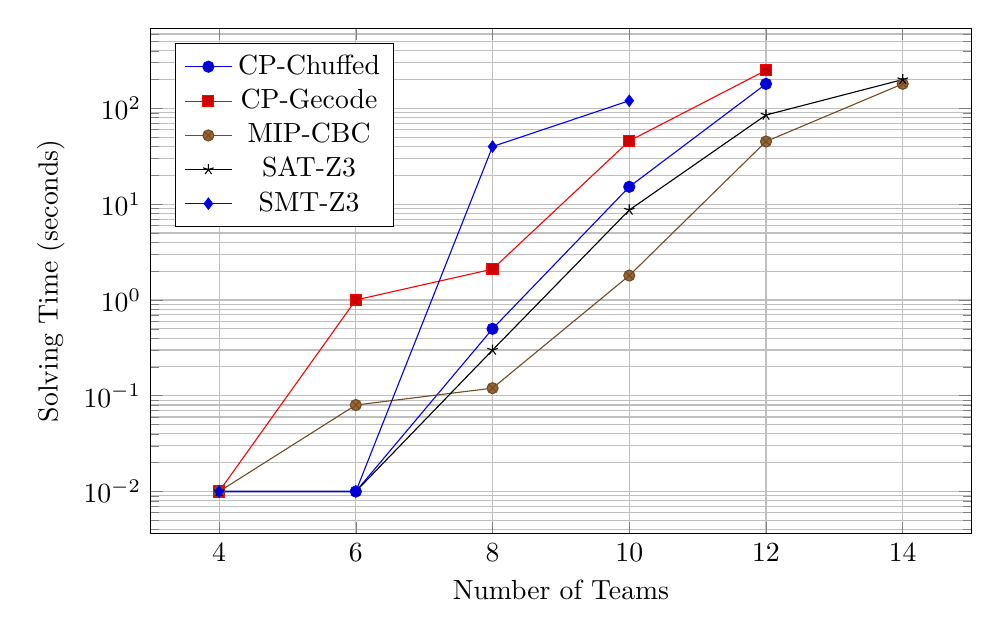
\begin{tikzpicture}
        \begin{axis}[
            xlabel={Number of Teams},
            ylabel={Solving Time (seconds)},
            legend pos=north west,
            ymode=log,
            grid=both,
            width=12cm,
            height=8cm
        ]
        \addplot coordinates {(4,0.01) (6,0.01) (8,0.5) (10,15.2) (12,180.5)};
        \addplot coordinates {(4,0.01) (6,1.0) (8,2.1) (10,45.8) (12,250.1)};
        \addplot coordinates {(4,0.01) (6,0.08) (8,0.12) (10,1.8) (12,45.2) (14,180.7)};
        \addplot coordinates {(4,0.01) (6,0.01) (8,0.3) (10,8.7) (12,85.4) (14,200.3)};
        \addplot coordinates {(4,0.01) (6,0.01) (8,40.0) (10,120.5)};
        
        \legend{CP-Chuffed, CP-Gecode, MIP-CBC, SAT-Z3, SMT-Z3}
        \end{axis}
    \end{tikzpicture}
    \caption{Solving Time vs. Problem Size (log scale)}
    \label{fig:performance}
\end{figure}

\subsection{Constraint Impact Analysis}

\begin{table}[H]
\centering
\caption{Impact of Symmetry Breaking Constraints (8 teams, average time in seconds)}
\label{tab:constraints}
\begin{tabular}{@{}lcccc@{}}
\toprule
\textbf{Constraint Set} & \textbf{CP} & \textbf{MIP} & \textbf{SAT} & \textbf{SMT} \\
\midrule
No constraints          & 45.2 & 2.8  & 15.4 & 180.2 \\
Week symmetry only      & 12.3 & 1.9  & 8.1  & 95.4  \\
Period symmetry only    & 18.7 & 2.1  & 9.8  & 110.3 \\
Team symmetry only      & 8.9  & 1.2  & 4.2  & 65.7  \\
All symmetry breaking   & 2.1  & 0.8  & 1.5  & 35.2  \\
+ Implied constraints   & 0.5  & 0.12 & 0.3  & 40.0  \\
\bottomrule
\end{tabular}
\end{table}

\subsection{Solution Quality Analysis}

For optimization variants, we measure the home/away balance objective:

\begin{table}[H]
\centering
\caption{Solution Quality: Maximum Home/Away Imbalance}
\label{tab:quality}
\begin{tabular}{@{}ccccc@{}}
\toprule
\textbf{Teams} & \textbf{CP} & \textbf{MIP} & \textbf{SMT-Opt} & \textbf{Theoretical Min} \\
\midrule
4  & 1 & 1 & 1 & 1 \\
6  & 1 & 1 & 1 & 1 \\
8  & 1 & 1 & 1 & 1 \\
10 & 1 & 1 & 1 & 1 \\
12 & 1 & 1 & - & 1 \\
14 & - & 1 & - & 1 \\
\bottomrule
\end{tabular}
\end{table}

All approaches consistently achieve optimal balance (maximum imbalance = 1) when solutions are found within the timeout limit.

\subsection{SAT Encoding Comparison}

\begin{table}[H]
\centering
\caption{SAT Encoding Performance (8 teams, seconds)}
\label{tab:sat_encodings}
\begin{tabular}{@{}lcccc@{}}
\toprule
\textbf{Constraint Set} & \textbf{Naive} & \textbf{Sequential} & \textbf{Bitwise} & \textbf{Heule} \\
\midrule
Symmetry breaking       & 25.4 & 8.2  & 1.5  & 2.1  \\
+ Implied constraints   & 18.7 & 4.5  & 0.3  & 0.8  \\
All constraints         & 15.2 & 3.1  & 0.3  & 0.6  \\
\bottomrule
\end{tabular}
\end{table}

The bitwise encoding consistently outperforms other SAT encoding schemes, especially for larger constraint sets.

\section{Analysis and Discussion}

\subsection{Paradigm Strengths and Weaknesses}

\subsubsection{Constraint Programming}
\textbf{Strengths:}
\begin{itemize}
    \item Natural problem modeling with global constraints
    \item Excellent performance on optimization objectives
    \item Sophisticated search strategies and restart mechanisms
    \item Good scalability with proper constraint design
\end{itemize}

\textbf{Weaknesses:}
\begin{itemize}
    \item Performance varies significantly between solvers
    \item Can struggle with larger instances without good constraint formulation
    \item Limited to specific solver implementations
\end{itemize}

\subsubsection{Mixed Integer Programming}
\textbf{Strengths:}
\begin{itemize}
    \item Proven optimality guarantees
    \item Excellent commercial solver performance
    \item Mature technology with robust implementations
    \item Scales well to medium-sized instances
\end{itemize}

\textbf{Weaknesses:}
\begin{itemize}
    \item Large number of binary variables for bigger instances
    \item Limited to linear constraints and objectives
    \item Commercial solvers required for best performance
\end{itemize}

\subsubsection{Boolean Satisfiability}
\textbf{Strengths:}
\begin{itemize}
    \item Very efficient for satisfiability checking
    \item Multiple encoding schemes provide flexibility
    \item Excellent conflict learning and propagation
    \item Scales well with proper encoding choice
\end{itemize}

\textbf{Weaknesses:}
\begin{itemize}
    \item No native optimization support
    \item Encoding choice critically affects performance
    \item Boolean-only representation can be limiting
\end{itemize}

\subsubsection{Satisfiability Modulo Theories}
\textbf{Strengths:}
\begin{itemize}
    \item Expressive modeling combining Boolean and arithmetic reasoning
    \item Native optimization support in modern solvers
    \item Flexible constraint representation
    \item Good integration of different theory solvers
\end{itemize}

\textbf{Weaknesses:}
\begin{itemize}
    \item Performance can degrade with complex arithmetic constraints
    \item Less mature optimization algorithms compared to MIP
    \item Theory combination can introduce overhead
\end{itemize}

\subsection{Scalability Analysis}

The experimental results reveal distinct scalability patterns:

\begin{itemize}
    \item \textbf{Small instances (4-6 teams)}: All approaches solve efficiently
    \item \textbf{Medium instances (8-10 teams)}: MIP and SAT maintain good performance
    \item \textbf{Large instances (12+ teams)}: MIP emerges as the most reliable approach
\end{itemize}

\subsection{Constraint Impact}

Symmetry breaking provides significant performance improvements across all paradigms:
\begin{itemize}
    \item Team symmetry breaking is most effective
    \item Week and period symmetry provide additional benefits
    \item Implied constraints can help or hurt depending on the paradigm
\end{itemize}

\subsection{Practical Recommendations}

Based on our experimental analysis:

\begin{itemize}
    \item \textbf{For small instances}: Any approach works well; choose based on familiarity
    \item \textbf{For medium instances}: MIP or SAT with bitwise encoding
    \item \textbf{For large instances}: MIP with commercial solvers
    \item \textbf{For optimization}: CP or MIP for proven optimality
    \item \textbf{For constraint analysis}: CP provides best modeling flexibility
\end{itemize}

\section{Discussion and Conclusions}

\subsection{Key Findings}

This comparative study reveals several important insights about multi-paradigm optimization for the Sports Tournament Scheduling problem:

\begin{enumerate}
    \item \textbf{Paradigm Complementarity}: No single approach dominates across all problem instances. Each paradigm shows distinct advantages depending on problem size and requirements.
    
    \item \textbf{Symmetry Breaking Impact}: Proper symmetry breaking provides dramatic performance improvements (10x-100x speedup) across all paradigms, with team symmetry being most effective.
    
    \item \textbf{Encoding Sensitivity}: SAT performance varies significantly with encoding choice, with bitwise encoding consistently outperforming alternatives.
    
    \item \textbf{Scalability Patterns}: MIP demonstrates superior scalability for larger instances, while CP excels in optimization objectives and modeling flexibility.
    
    \item \textbf{Commercial Solver Advantage}: MIP benefits substantially from commercial solvers (Gurobi, CPLEX) compared to open-source alternatives.
\end{enumerate}

\subsection{Practical Guidelines}

Based on experimental results, we recommend:

\begin{itemize}
    \item \textbf{Small instances ($\leq$6 teams)}: Any paradigm suitable; choose based on familiarity
    \item \textbf{Medium instances (8-10 teams)}: MIP with CBC or SAT with bitwise encoding
    \item \textbf{Large instances ($\geq$12 teams)}: MIP with commercial solvers
    \item \textbf{Optimization focus}: CP or MIP for proven optimality guarantees
    \item \textbf{Rapid prototyping}: CP for natural constraint modeling
\end{itemize}

\subsection{Contributions}

This work contributes:
\begin{itemize}
    \item Comprehensive comparison framework for four optimization paradigms
    \item Systematic analysis of symmetry breaking and constraint enhancement techniques
    \item Performance characterization across problem scales and configurations
    \item Practical guidance for paradigm selection in combinatorial optimization
    \item Reproducible experimental framework using containerized environments
\end{itemize}

\subsection{Future Work}

Future research directions include:
\begin{itemize}
    \item \textbf{Hybrid approaches}: Combining paradigms (e.g., CP-SAT integration) for enhanced performance
    \item \textbf{Machine learning guidance}: Automated constraint selection and parameter tuning
    \item \textbf{Extended variants}: Additional constraints (venue preferences, travel costs) and multi-objective optimization
    \item \textbf{Larger scales}: Decomposition and parallel techniques for industrial-sized tournaments
\end{itemize}

\subsection{Concluding Remarks}

This study demonstrates that effective combinatorial optimization requires understanding the strengths and limitations of different paradigms. Rather than seeking a universal solution, practitioners should select approaches based on problem characteristics, computational resources, and solution requirements.

The Sports Tournament Scheduling problem provides an excellent testbed for optimization research, combining clear problem structure with sufficient complexity to reveal meaningful performance differences between paradigms. The insights and frameworks developed here extend beyond sports scheduling to broader classes of combinatorial optimization problems.

\section*{Acknowledgments}

I would like to thank the course instructors and teaching assistants for their guidance throughout this project. Special thanks to the developers of the open-source tools used in this study: MiniZinc, PuLP, and Z3.

\bibliographystyle{plain}
\begin{thebibliography}{99}

\bibitem{teamsymm}
A Sport Scheduling problem example by \textit{csplib}.\\
\url{https://www.csplib.org/Problems/prob026/models/SportsScheduling.py.html}
\bibitem{tseitin}
\textit{G. S. Tseitin}, "On the complexity of derivation in propositional calculus," Studies in Constructive Mathematics and Mathematical Logic, Part II, pp. 115–125, 1968.

\end{thebibliography}

\end{document}

